\documentclass[10pt]{article}
\usepackage[margin=0.75in]{geometry}
\usepackage{amsmath,amssymb}
\usepackage{xcolor}
\usepackage{tikz}
\usepackage[most]{tcolorbox}
\usepackage{enumitem}
\usepackage{titlesec}
\usepackage{fancyhdr}

\definecolor{ink}{HTML}{1F3A5F}
\definecolor{key}{HTML}{8A1C1C}
\definecolor{soft}{HTML}{EEF3F8}
\definecolor{warm}{HTML}{FBF3E6}

\setlength{\parindent}{0pt}
\setlength{\parskip}{4pt}
\setlist{itemsep=1pt,topsep=2pt}
\titleformat{\section}{\large\bfseries\color{ink}}{\thesection.}{0.5em}{}
\titleformat{\subsection}{\normalsize\bfseries\color{ink}}{}{0em}{}
\titlespacing*{\section}{0pt}{10pt}{4pt}
\titlespacing*{\subsection}{0pt}{6pt}{2pt}

\newcommand{\E}{\mathrm{E}}

\newtcolorbox{bigidea}{colback=soft,colframe=ink,boxrule=0.6pt,arc=2pt,left=5pt,right=5pt,top=3pt,bottom=3pt,
  title={\bfseries\small Big idea},fonttitle=\small}
\newtcolorbox{trap}{colback=warm,colframe=key,boxrule=0.6pt,arc=2pt,left=5pt,right=5pt,top=3pt,bottom=3pt,
  title={\bfseries\small Traps / what graders look for},fonttitle=\small}
\newtcolorbox{answer}{colback=white,colframe=ink,boxrule=0.6pt,arc=2pt,left=6pt,right=6pt,top=4pt,bottom=4pt,
  title={\bfseries\small Model answer},fonttitle=\small,breakable}

\pagestyle{fancy}
\fancyhf{}
\renewcommand{\headrulewidth}{0pt}
\fancyfoot[C]{\small\thepage}

% Shared TikZ figures for the ECON 5040 midterm study guide and sample midterm.
% Each \fig... macro draws one self-contained tikzpicture.

% 1. Intertemporal budget line: R is minus the slope
\newcommand{\figIntertemporal}{%
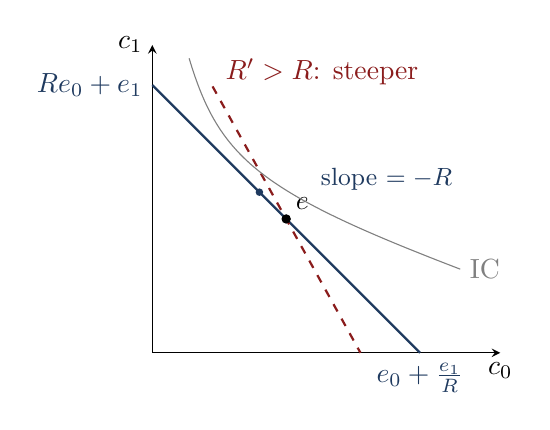
\begin{tikzpicture}[scale=0.85,>=stealth]
  \draw[->] (0,0) -- (5.2,0) node[below] {$c_0$};
  \draw[->] (0,0) -- (0,4.6) node[left] {$c_1$};
  % endowment e = (2,2); budget with R = 1 (slope -1) and R' > R (slope -1.8)
  \draw[thick,ink] (0,4) -- (4,0) node[below] {$e_0+\tfrac{e_1}{R}$};
  \node[left,ink] at (0,4) {$Re_0+e_1$};
  \draw[thick,key,dashed] (0.9,3.98) -- (3.11,0);
  \node[key,right] at (0.95,4.2) {$R'>R$: steeper};
  \fill (2,2) circle (2pt) node[above right] {$e$};
  % indifference curve tangent to the original line at (1.6,2.4)
  \draw[gray] (0.55,4.4) .. controls (1.0,2.9) and (1.6,2.4) .. (4.6,1.25);
  \fill[ink] (1.6,2.4) circle (1.6pt);
  \node[gray,right] at (4.6,1.25) {IC};
  \node[ink] at (3.5,2.6) {\small slope $=-R$};
\end{tikzpicture}}

% 2. Concave utility, expected utility, certainty equivalent
\newcommand{\figCE}{%
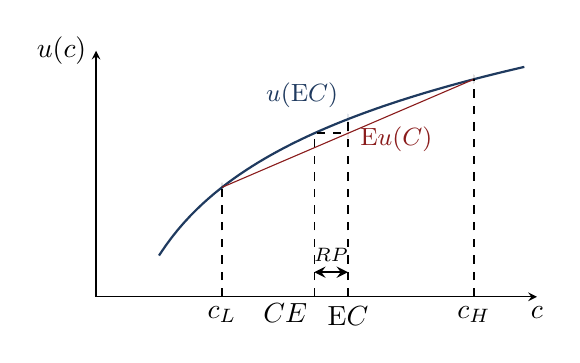
\begin{tikzpicture}[xscale=0.032,yscale=1.25,>=stealth]
  \draw[->] (0,2.8) -- (175,2.8) node[below] {$c$};
  \draw[->] (0,2.8) -- (0,5.3) node[left] {$u(c)$};
  \draw[thick,ink,domain=25:170,samples=60] plot (\x,{ln(\x)});
  \draw[key] (50,{ln(50)}) -- (150,{ln(150)});
  \fill (50,{ln(50)}) circle (1.4pt); \fill (150,{ln(150)}) circle (1.4pt);
  % E[C]=100, E[u]=0.5(ln50+ln150)=4.4637, CE=86.6, u(100)=4.6052
  \fill[key] (100,4.4637) circle (1.6pt);
  \fill[ink] (100,4.6052) circle (1.6pt);
  \draw[dashed] (100,2.8) node[below] {$\E C$} -- (100,4.6052);
  \draw[dashed] (86.6,2.8) node[below left=-1pt] {$CE$} -- (86.6,4.4637) -- (100,4.4637);
  \draw[dashed] (50,2.8) node[below] {$c_L$} -- (50,{ln(50)});
  \draw[dashed] (150,2.8) node[below] {$c_H$} -- (150,{ln(150)});
  \node[ink,above left] at (100,4.62) {\small $u(\E C)$};
  \node[key,right] at (101,4.40) {\small $\E u(C)$};
  \draw[<->,thick] (86.6,3.05) -- node[above] {\scriptsize $RP$} (100,3.05);
\end{tikzpicture}}

% 3. Two-state Markov chain
\newcommand{\figMarkov}{%
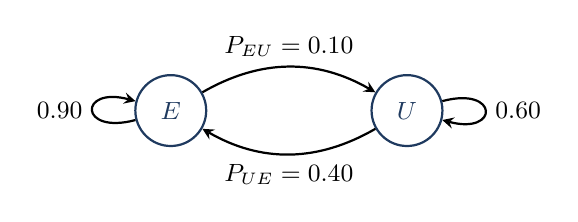
\begin{tikzpicture}[>=stealth,node distance=3cm,every node/.style={font=\small}]
  \node[circle,draw,thick,ink,minimum size=9mm] (E) {$E$};
  \node[circle,draw,thick,ink,minimum size=9mm,right of=E] (U) {$U$};
  \draw[->,thick] (E) to[bend left] node[above] {$P_{EU}=0.10$} (U);
  \draw[->,thick] (U) to[bend left] node[below] {$P_{UE}=0.40$} (E);
  \draw[->,thick] (E) to[loop left] node[left] {$0.90$} (E);
  \draw[->,thick] (U) to[loop right] node[right] {$0.60$} (U);
\end{tikzpicture}}

% 4. Bellman decomposition / timing
\newcommand{\figBellman}{%
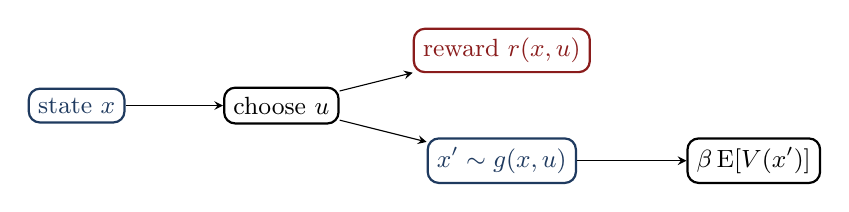
\begin{tikzpicture}[>=stealth,every node/.style={font=\small}]
  \node[draw,rounded corners,ink,thick] (x) at (0,0) {state $x$};
  \node[draw,rounded corners,thick] (u) at (2.6,0) {choose $u$};
  \node[draw,rounded corners,key,thick] (r) at (5.4,0.7) {reward $r(x,u)$};
  \node[draw,rounded corners,ink,thick] (xp) at (5.4,-0.7) {$x'\sim g(x,u)$};
  \node[draw,rounded corners,thick] (v) at (8.6,-0.7) {$\beta\,\E[V(x')]$};
  \draw[->] (x) -- (u); \draw[->] (u) -- (r); \draw[->] (u) -- (xp); \draw[->] (xp) -- (v);
\end{tikzpicture}}

% 5. Solow: sf(k) vs delta k, with a rise in s
\newcommand{\figSolow}{%
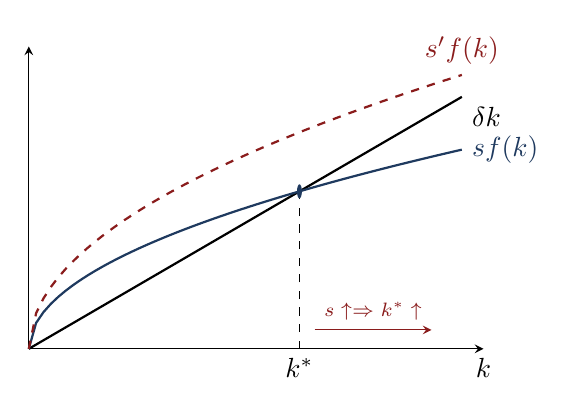
\begin{tikzpicture}[xscale=0.55,yscale=1.6,>=stealth]
  \draw[->] (0,0) -- (10.5,0) node[below] {$k$};
  \draw[->] (0,0) -- (0,2.4);
  \draw[thick] (0,0) -- (10,2) node[below right] {$\delta k$};
  \draw[thick,ink,domain=0:10,samples=60] plot (\x,{0.4*sqrt(\x)*1.25}) node[right] {$sf(k)$};
  \draw[thick,key,dashed,domain=0:10,samples=60] plot (\x,{0.55*sqrt(\x)*1.25}) node[above] {$s'f(k)$};
  % k* where 0.5 sqrt k = 0.2 k -> k = 6.25 ; k*' where 0.6875 sqrt k = 0.2k -> k = 11.8 (off-axis) so use 0.55*1.25=0.6875
  \draw[dashed] (6.25,0) node[below] {$k^*$} -- (6.25,1.25);
  \fill[ink] (6.25,1.25) circle (1.6pt);
  \draw[->,key] (6.6,0.15) -- (9.3,0.15) node[midway,above] {\scriptsize $s\uparrow\Rightarrow k^*\uparrow$};
  
\end{tikzpicture}}

% 6. Level effect vs growth effect
\newcommand{\figLevelGrowth}{%
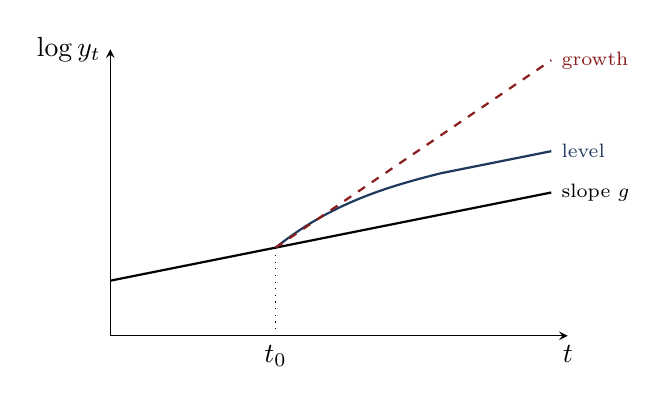
\begin{tikzpicture}[xscale=0.7,yscale=0.7,>=stealth]
  \draw[->] (0,0) -- (8.3,0) node[below] {$t$};
  \draw[->] (0,0) -- (0,5.2) node[left] {$\log y_t$};
  \draw[thick] (0,1) -- (8,2.6) node[right] {\scriptsize slope $g$};
  \draw[thick,ink] (3,1.6) .. controls (4,2.4) and (5,2.7) .. (6,2.95) -- (8,3.35) node[right] {\scriptsize level};
  \draw[thick,key,dashed] (3,1.6) -- (8,5.0) node[right] {\scriptsize growth};
  \draw[dotted] (3,0) node[below] {$t_0$} -- (3,1.6);
\end{tikzpicture}}

% 7. Convex marginal utility -> precautionary saving
\newcommand{\figPrecaution}{%
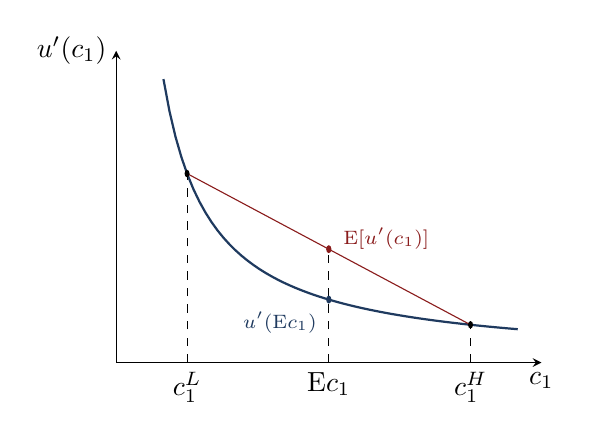
\begin{tikzpicture}[xscale=0.6,yscale=0.9,>=stealth]
  \draw[->] (0,0) -- (9,0) node[below] {$c_1$};
  \draw[->] (0,0) -- (0,4.4) node[left] {$u'(c_1)$};
  \draw[thick,ink,domain=1:8.5,samples=60] plot (\x,{4/\x});
  \draw[key] (1.5,2.667) -- (7.5,0.533);
  \fill (1.5,2.667) circle (1.5pt); \fill (7.5,0.533) circle (1.5pt);
  \draw[dashed] (1.5,0) node[below] {$c_1^L$} -- (1.5,2.667);
  \draw[dashed] (7.5,0) node[below] {$c_1^H$} -- (7.5,0.533);
  \draw[dashed] (4.5,0) node[below] {$\E c_1$} -- (4.5,1.6);
  \fill[key] (4.5,1.6) circle (1.6pt); \fill[ink] (4.5,0.889) circle (1.6pt);
  \node[key,right] at (4.6,1.75) {\scriptsize $\E[u'(c_1)]$};
  \node[ink,below left] at (4.45,0.85) {\scriptsize $u'(\E c_1)$};
\end{tikzpicture}}

% 8. McCall reservation wage
\newcommand{\figMcCall}{%
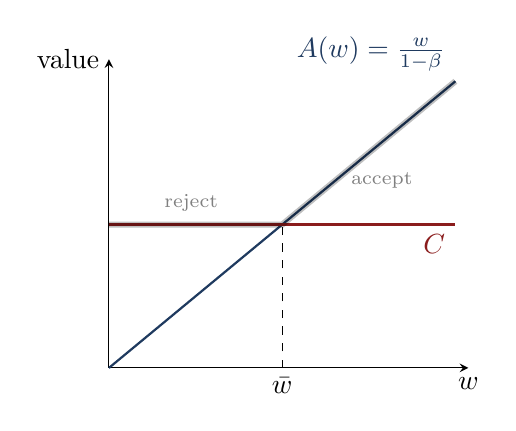
\begin{tikzpicture}[xscale=0.55,yscale=0.7,>=stealth]
  \draw[->] (0,0) -- (8.3,0) node[below] {$w$};
  \draw[->] (0,0) -- (0,5.6) node[left] {value};
  \draw[thick,ink] (0,0) -- (8,5.2) node[above left] {$A(w)=\frac{w}{1-\beta}$};
  \draw[thick,key] (0,2.6) -- (8,2.6) node[below left] {$C$};
  \draw[dashed] (4,0) node[below] {$\bar w$} -- (4,2.6);
  \draw[line width=2.2pt,opacity=0.25] (0,2.6) -- (4,2.6) -- (8,5.2);
  \node[gray] at (1.9,3.0) {\scriptsize reject};
  \node[gray] at (6.3,3.4) {\scriptsize accept};
\end{tikzpicture}}


\begin{document}

\begin{center}
{\LARGE\bfseries\color{ink} ECON 5040 Midterm: Comprehensive Study Guide}\\[3pt]
{\small Dynamic Stochastic Modeling (Fisher), Fall 2026. Covers all 10 topics on the official study guide, in Fisher's notation.\\
The exam is closed book: one question per topic, answered in 3--4 sentences plus maybe a graph. The worked answers are in \texttt{ECON5040\_Sample\_Midterm.pdf}.}
\end{center}

\begin{tcolorbox}[colback=soft,colframe=ink,boxrule=0.6pt,arc=2pt,title={\bfseries How to write a full-credit answer (every topic)},fonttitle=\small]
\small
\textbf{(1)} State the central idea in one sentence. \textbf{(2)} Write the key equation and say what \emph{each side} means economically. \textbf{(3)} Give the mechanism or comparative static (``if $X$ rises, then \dots\ because \dots''). \textbf{(4)} Add a labeled graph if one exists for the topic. Fisher says \emph{not} to memorize long derivations or code; he grades whether you can interpret the equations and explain how the pieces fit together.
\end{tcolorbox}

%==================================================================
\section{Inter-temporal Prices}

\begin{bigidea}
Consumption today ($c_0$) and consumption next year ($c_1$) are \emph{different commodities}. The gross real interest rate $R=1+r$ is the relative price between them: give up 1 unit today and you get $R$ units tomorrow.
\end{bigidea}

\begin{minipage}{0.56\textwidth}
\textbf{Prices.} Set today's good as the numéraire, $p_0=1$. The price today of one unit of future consumption is $p_1=1/R$, so $R=p_0/p_1$: the price of current consumption in units of future consumption.

\textbf{Budget.} With endowment $(e_0,e_1)$: $c_0+\dfrac{c_1}{R}=e_0+\dfrac{e_1}{R}$ (present value of wealth). The budget line has slope $-R$ and passes through the endowment.

\textbf{Optimality (interior).} MRS $=$ relative price:
\[\frac{u'(c_0)}{\beta u'(c_1)}=R.\]
The left side is how many units of $c_1$ you need to give up one unit of $c_0$; the right side is how many the market gives you.
\end{minipage}\hfill
\begin{minipage}{0.4\textwidth}\centering
\figIntertemporal
\end{minipage}

\textbf{Substitution incentive.} A rise in $R$ makes future consumption \emph{cheaper} (its price $1/R$ falls) and current consumption more expensive. The substitution effect therefore always pushes the household to consume less today and save more. Graphically, the budget line pivots \emph{through the endowment} and gets steeper. With CRRA utility, $c_1/c_0=(\beta R)^{1/\rho}$, so $1/\rho$ measures how strongly the household substitutes (the elasticity of intertemporal substitution).

\textbf{Income/wealth effect (for completeness).} A lender (with $c_0<e_0$) becomes richer when $R$ rises, which pushes $c_0$ up. A borrower becomes poorer. So the \emph{total} effect on saving is ambiguous for a lender, but the substitution effect alone is unambiguous.

\textbf{Time separability.} $U=\sum_t\beta^tu(c_t)$. Here $\beta$ is impatience, and $u$ (``felicity'') has the same shape every period. Separability means the MRS between $t$ and $t+1$ does not depend on consumption at other dates (Fisher's breakfast/lunch/dinner example). It is restrictive but tractable.

\begin{trap}
\small Say ``relative price'' explicitly. $R$ is a price, not just a return. A higher $R$ makes the \emph{future} cheap. Don't claim saving \emph{must} rise; that holds for the substitution effect only.
\end{trap}

%==================================================================
\section{Choice Under Uncertainty}

\begin{bigidea}
Under the vNM axioms (completeness, transitivity, continuity, independence), lotteries are ranked by \textbf{expected utility} $\E[u(C)]=\sum_s\pi_su(c_s)$. The \emph{curvature} of $u$ encodes the attitude toward risk.
\end{bigidea}

\begin{minipage}{0.52\textwidth}
\textbf{Risk aversion.} $u$ concave ($u''<0$) $\iff u(\E C)\ge\E u(C)$ (Jensen). Marginal utility is diminishing, so a bad outcome hurts more than an equal-sized good outcome helps.

\textbf{Certainty equivalent.} $u(CE)=\E u(C)$, so $CE=u^{-1}(\E u(C))$. This is the sure amount the consumer values the same as the gamble. It satisfies $CE<\E C$ when the consumer is risk averse.

\textbf{Risk premium.} $RP=\E C-CE$: the expected consumption the consumer would give up to remove the risk.
\end{minipage}\hfill
\begin{minipage}{0.45\textwidth}\centering
\figCE
\end{minipage}

\textbf{Canonical example (memorize).} $u=\log c$, with $C=50$ or $150$ each with probability $\tfrac12$. Then $\E C=100$, and
$\log CE=\tfrac12\log50+\tfrac12\log150\Rightarrow CE=\sqrt{50\cdot150}=\sqrt{7500}\approx\mathbf{86.60}$, so $RP\approx13.40$.\\
General recipe: (1) compute $\E u$; (2) invert $u$. With log utility, $CE$ is the \emph{geometric mean} of the outcomes.

\textbf{Curvature measures.} The coefficient of absolute risk aversion is $A(c)=-u''/u'$ (for fixed-dollar gambles). The coefficient of relative risk aversion is $\rho(c)=-cu''/u'$ (for percentage gambles). Under CRRA, $u=\frac{c^{1-\rho}-1}{1-\rho}$, $\rho$ is constant; log is the case $\rho=1$, with $A=1/c$ (decreasing). More curvature gives a lower $CE$ and a bigger $RP$. A risk-neutral consumer (linear $u$) has $CE=\E C$.

\textbf{vNM vs.\ ordinary utility.} vNM utility is unique only up to a \emph{positive affine} transformation $a+bu$; an arbitrary increasing transformation would change how lotteries are ranked.

\begin{trap}
\small Don't compute $u(\E C)$ and call it the CE. The CE comes from inverting \emph{expected} utility. Always state the inequality $CE<\E C$ and say it is \emph{because} $u$ is concave.
\end{trap}

%==================================================================
\section{Markov Processes}

\begin{bigidea}
\textbf{Markov property:} $\Pr(X_{t+1}=j\mid X_t=i,X_{t-1},\dots,X_0)=\Pr(X_{t+1}=j\mid X_t=i)$. Once you know today's state, the earlier history adds nothing to the forecast of tomorrow. History still matters, but \emph{only through} the current state.
\end{bigidea}

\begin{minipage}{0.55\textwidth}
\textbf{Transition matrix.} $P_{ij}=\Pr(X_{t+1}=j\mid X_t=i)$. Rows are today's state and columns are tomorrow's.
\begin{itemize}
\item \textbf{Element $P_{ij}$:} the probability of moving to $j$ next period given you are in $i$ now. Example: with $P=\begin{bmatrix}.9&.1\\.4&.6\end{bmatrix}$ ($E$, $U$), $P_{UE}=0.4$ is the \emph{job-finding rate} and $P_{EU}=0.1$ is the \emph{job-separation rate}.
\item \textbf{Row $i$:} the entire conditional distribution of tomorrow's state given $i$ today. It is non-negative and sums to 1 (a stochastic matrix).
\end{itemize}
\end{minipage}\hfill
\begin{minipage}{0.42\textwidth}\centering
\figMarkov
\end{minipage}

\textbf{Distributions.} Write the distribution as a row vector $\psi_t$. It evolves by $\psi_{t+1}=\psi_tP$, so $\psi_t=\psi_0P^t$, and $(P^n)_{ij}=\Pr(X_{t+n}=j\mid X_t=i)$. For example, $(P^2)_{EU}=.9(.1)+.1(.6)=0.15$.\\
\textbf{Stationary distribution.} $\psi^*=\psi^*P$. In the example, $u=.1(1-u)+.6u\Rightarrow u^*=0.2$, so $\psi^*=(0.8,0.2)$. Individuals keep moving between states, but the \emph{shares} stay constant. Long-run simulated frequencies approach $\psi^*$ (LLN).

\textbf{Why it matters later.} In a DP, the state's transition is a Markov chain that can depend on the action ($M_u$). Once you fix an optimal policy $h$, it induces its own chain $P_h(x,\cdot)=M_{h(x)}(x,\cdot)$.

%==================================================================
\section{Introduction to Dynamic Programming}

\begin{bigidea}
``What we choose now changes our future irrevocably.'' The \textbf{Bellman equation} splits an infinite-horizon problem into \emph{today's reward} plus the \emph{discounted expected value of where you end up}:
\[V(x)=\max_{u\in U}\Big\{\underbrace{r(x,u)}_{\text{reward today}}+\beta\,\underbrace{\E[V(x')\mid x,u]}_{\text{continuation value}}\Big\},\qquad x'\sim g(x,u).\]
\end{bigidea}

\textbf{The five ingredients:} the state space $X$, the control set $U$, the reward $r(x,u)$, the (random) transition $x'\sim g(x,u)$, and the discount factor $\beta\in[0,1)$. The original problem is $\max\E\sum_t\beta^tr(x_t,u_t)$. The Bellman equation replaces choosing an infinite sequence with choosing \emph{one} action today, given $V$. The catch is that $V$ appears on both sides, so it is a \emph{fixed-point} equation.

\begin{center}\figBellman\end{center}

\textbf{How to identify the pieces (practice table).}

{\small
\begin{tabular}{@{}lllll@{}}
\hline
Problem & State $x$ & Choice $u$ & Current payoff & Next state $x'$\\ \hline
Optimal growth & $k_t$ & $k_{t+1}$ & $\log(Ak^\alpha-k')$ & $k'=u$\\
Cake eating & $x_t$ (cake) & $c_t$ & $u(c)$ & $x'=x-c$\\
Student TV/Study & health & TV / Study & $r(x,u)$ table & $x'\sim M_u(x,\cdot)$\\
McCall search & offer $w$ & accept / reject & $w$ or $c$ & $W'\sim F$ (if reject)\\
Income fluctuation & $(a,z)$ & $a'$ (or $c$) & $u(Ra+y(z)-a')$ & $(a',z')$, $z'\sim P(z,\cdot)$\\ \hline
\end{tabular}}

\textbf{The state} is \emph{everything you need today} to make the decision and to forecast tomorrow. It is a ``sufficient statistic'' for the past, which is the Markov idea. \textbf{The choice} is what the agent controls. The control can affect today's reward, tomorrow's state, or both.

\textbf{Worked example (optimal growth).} $V(k)=\max_{k'}\{\log(Ak^\alpha-k')+\beta V(k')\}$. Guess $V=E+F\log k$ and verify: $F=\alpha/(1-\alpha\beta)$, giving the policy $k'=\alpha\beta Ak^\alpha$ (save the constant fraction $\alpha\beta$ of output). The steady state is $k^*=(\alpha\beta A)^{1/(1-\alpha)}$.

%==================================================================
\section{Value Functions and Policy Functions}

\begin{bigidea}
\textbf{Value function} $V(x)$: ``How good is it to be here right now, knowing my future plans are as good as can be?'' It is a \emph{number} for each state (lifetime utility).\\
\textbf{Policy function} $h(x)$: ``What should I do, come what may?'' It is an \emph{action} for each state (a contingent plan).
\end{bigidea}

\begin{itemize}
\item In a stochastic world the solution cannot be a fixed sequence $(u_0,u_1,\dots)$, because future states are unknown. It has to be a \emph{rule}, $u_t=h(x_t)$.
\item \textbf{The link:} the policy is the argmax of the Bellman equation, \[h(x)=\arg\max_u\{r(x,u)+\beta\E[V(x')\mid x,u]\},\] and the value is what you get by following it: $V(x)=r(x,h(x))+\beta\E[V(x')\mid x,h(x)]$. Know $V$ and you get $h$ from one maximization. Know $h$ and you get $V_h$ by solving a linear system.
\item \textbf{Economic information:} $V$ measures welfare and the value of resources. $V'(x)$ is the shadow value of one more unit of the state; by the envelope condition $V'(x)=u'(c)$ in cake eating and $u'(c)f'(k)$ in growth. $h$ gives \emph{behavior}: the saving rule, the reservation-wage rule, the law of motion $k'=h(k)$, and the Markov chain $P_h$ that drives long-run outcomes.
\item Examples: in cake eating $V(x)$ is maximal lifetime utility and $c^*(x)=(1-\beta^{1/\rho})x$; in McCall $V(w)=\max\{A(w),C\}$ and $h(w)=$ accept iff $w\ge\bar w$; in growth $h(k)=\alpha\beta Ak^\alpha$.
\end{itemize}
\textbf{Chain to remember:} dynamic problem $\to$ Bellman equation $\to$ value function $\to$ policy function $\to$ law of motion / Markov chain $\to$ long-run outcomes.

%==================================================================
\section{Howard's Method versus Value Function Iteration}

\begin{bigidea}
Both methods solve the same Bellman equation. \textbf{VFI} starts from a guessed \emph{value function} and iterates $V_{n+1}=TV_n$. \textbf{Howard} starts from a guessed \emph{policy} and alternates \emph{exact policy evaluation} with \emph{policy improvement}.
\end{bigidea}

\textbf{VFI.} The Bellman operator is $(TV)(x)=\max_u\{r(x,u)+\beta\sum_{x'}M_u(x,x')V(x')\}$. Start at $V_0=0$, so $V_1=\max_ur(x,u)$ (only today counts). Each application of $T$ adds one more period of future rewards. Stop when $\|V_{n+1}-V_n\|$ is tiny, then read off $h=\arg\max$. $T$ is a contraction with modulus $\beta$, so the error shrinks by a factor $\approx\beta$ per step. That is \emph{slow when $\beta$ is close to 1}: hundreds of iterations, each requiring a full maximization.

\textbf{Howard (policy iteration).}
\begin{enumerate}[leftmargin=*]
\item Guess a policy $h_0$.
\item \textbf{Evaluate:} with the policy fixed, the max disappears and $V_h=r_h+\beta P_hV_h\Rightarrow V_h=(I-\beta P_h)^{-1}r_h$. This is one linear solve.
\item \textbf{Improve:} $h_1(x)=\arg\max_uQ(x,u;V_{h_0})$, where $Q=r(x,u)+\beta\sum M_u(x,x')V_{h_0}(x')$.
\item Stop when the policy doesn't change; otherwise repeat.
\end{enumerate}
\textbf{Why Howard is faster.} The evaluation step computes the value of following $h$ \emph{forever} in one shot, which is equivalent to infinitely many VFI steps with the policy held fixed. Each improvement step then makes a big jump. There are only finitely many policies ($|U|^{|X|}$, e.g.\ $2^3=8$ for the student) and each round weakly improves, so it converges in a \emph{handful} of iterations. The trade-off is that each iteration costs a linear solve.

\textbf{Student example} ($\beta=.5$, $h_0=$ TV everywhere): $V_{h_0}\approx(3.64,\,6.92,\,13.40)$. The improvement check gives TV in every state (e.g.\ Sick: TV $3.64$ vs.\ Study $0.98$), so the guess was already optimal and the method stops after one round.

\begin{trap}
\small Key words: VFI = ``value guess, apply $T$ until $V$ converges.'' Howard = ``policy guess, \emph{evaluate} (a linear system), \emph{improve} (argmax), stop when the policy is unchanged.''
\end{trap}

%==================================================================
\section{The Solow Model}

\begin{bigidea}
The saving rate $s$ is \textbf{exogenous}. Capital accumulates according to $k_{t+1}=sf(k_t)+(1-\delta)k_t$. Diminishing returns ($f''<0$) mean investment eventually only covers depreciation, so the economy converges to a \textbf{steady state} $sf(k^*)=\delta k^*$.
\end{bigidea}

\begin{minipage}{0.52\textwidth}
\textbf{Steady state.} Investment equals replacement: $sf(k^*)=\delta k^*$. With $f=Ak^\alpha$,
\[k^*=\Big(\frac{sA}{\delta}\Big)^{\frac1{1-\alpha}},\quad y^*=A(k^*)^\alpha,\quad c^*=(1-s)y^*.\]
\textbf{Convergence.} If $k<k^*$ then $sf(k)>\delta k$ and $k$ rises; if $k>k^*$ it falls. In the 45° diagram, $k^*$ is where $g(k)$ crosses the 45° line.\\
\textbf{Comparative statics.} $s\uparrow$, $A\uparrow\Rightarrow k^*,y^*\uparrow$; $\delta\uparrow$ (or $n\uparrow$) $\Rightarrow k^*\downarrow$.
\end{minipage}\hfill
\begin{minipage}{0.45\textwidth}\centering
\figSolow
\end{minipage}

\begin{minipage}{0.52\textwidth}
\textbf{Level vs.\ growth (the key distinction).} A permanent rise in $s$ raises $k^*$ and $y^*$: a \textbf{level effect}. Growth is temporarily faster during the transition, but at the new steady state, per-worker growth returns to its old rate. Long-run growth of output per worker equals the rate of technical progress $g$, which comes from $E_{t+1}=(1+g)E_t$ (aggregate output grows at $n+g+ng$). Saving cannot permanently raise growth because diminishing returns choke off the extra investment. Only a change in $g$ (or ongoing increases in $A$) changes the \emph{slope} of $\log y_t$.
\end{minipage}\hfill
\begin{minipage}{0.45\textwidth}\centering
\figLevelGrowth
\end{minipage}

\textbf{Extras.}
\begin{itemize}
\item \textbf{Golden rule.} More saving need not raise $c^*=(1-s)f(k^*)$. With Cobb--Douglas, $s_{GR}=\alpha$, but Solow doesn't explain why households would pick it.
\item \textbf{Factor prices.} $r=\alpha Ak^{\alpha-1}-\delta$ falls with $k$, and $w=(1-\alpha)Ak^\alpha$ rises with $k$.
\item \textbf{Convergence speed.} $\lambda=1-\frac{(1-\alpha)(\delta+n+g+ng)}{(1+n)(1+g)}$, half-life $=\ln(1/2)/\ln\lambda\approx13$ years. Note that $s$ does not affect the speed.
\end{itemize}

%==================================================================
\section{Optimal Saving}

\begin{bigidea}
Saving is now a \emph{choice}. The \textbf{Euler equation}
\[\underbrace{u'(c_t)}_{\text{MU of eating 1 more unit today}}=\underbrace{\beta R\,\E_t[u'(c_{t+1})]}_{\text{discounted expected MU of saving it: }R\text{ units tomorrow}}\]
says that at the optimum, you can't gain by shifting one unit between today and tomorrow.
\end{bigidea}

\textbf{Derivation logic (cake eating, $R=1$).} $V(x)=\max_c\{u(c)+\beta V(x-c)\}$. The FOC is $u'(c_t)=\beta V'(x_{t+1})$ and the envelope condition is $V'(x)=u'(c)$. Together these give $u'(c_t)=\beta u'(c_{t+1})$. With CRRA, $c_{t+1}/c_t=(\beta R)^{1/\rho}$, and in cake eating the policy is $c^*(x)=(1-\beta^{1/\rho})x$ ($=(1-\beta)x$ for log). In the growth model, $R$ is replaced by $f'(k_{t+1})$: MRS $=$ marginal efficiency of investment $=$ gross real interest rate.

\textbf{When the two sides are not equal (the exam question).}
\begin{itemize}
\item $u'(c_t)>\beta R\E u'(c_{t+1})$: a unit eaten today is worth more than the same unit saved. The household should \textbf{consume more today and save less}. That lowers $u'(c_t)$ and raises $u'(c_{t+1})$ (since $c_{t+1}$ falls) until the two sides are equal.
\item $u'(c_t)<\beta R\E u'(c_{t+1})$: saving is worth more, so the household should \textbf{consume less today and save more}, until equality.
\item Exception: with a borrowing constraint $a'\ge\underline a$ that binds, the household \emph{wants} to consume more but can't, so $u'(c_t)>\beta R\E u'(c_{t+1})$ persists at the optimum (the Euler \emph{inequality}).
\end{itemize}
\textbf{Comparative statics.} $\beta\uparrow$ (more patient) means save more. $R\uparrow$ means a steeper consumption profile (substitution). If $\beta R<1$, consumption declines over time; if $\beta R=1$, it is flat (perfect smoothing).

%==================================================================
\section{Income Fluctuations}

\begin{bigidea}
With uninsurable income risk and incomplete markets, a risk-free asset is the only tool. Households \textbf{self-insure} by building a buffer of assets. \textbf{Precautionary saving} means uncertainty itself raises saving, even when \emph{expected} income is unchanged.
\end{bigidea}

\begin{minipage}{0.55\textwidth}
\textbf{Why (math).} Euler: $u'(c_0)=\beta R\E[u'(c_1)]$. If $u'$ is \emph{convex} ($u'''>0$, e.g.\ log, where $u'=1/c$), Jensen gives $\E[u'(c_1)]>u'(\E c_1)$. A mean-preserving spread in $Y_1$ therefore raises the right side at any given $a_1$. To restore equality the household must raise $u'(c_0)$, which means it must \textbf{save more}.\\
\textbf{Why (economics).} Bad states have very high marginal utility, so an extra dollar of assets is especially valuable when income turns out low.\\
\textbf{Classroom example:} $Y_1\in\{2,10\}$ vs.\ a certain $6$, with the same mean; the risky case saves more.
\end{minipage}\hfill
\begin{minipage}{0.42\textwidth}\centering
\figPrecaution
\end{minipage}

\textbf{Self-insurance.} The asset pays $R$ in \emph{every} state, so it is not state-contingent insurance. But consumption is chosen \emph{after} income is observed, so assets can be drawn down when income is low. The buffer transfers resources toward the future states where consumption and wealth are low. Three distinct ideas: \emph{smoothing} (dislike fluctuations), \emph{self-insurance} (the buffer), and \emph{precautionary saving} (risk raises saving relative to the no-risk benchmark).

\textbf{Infinite-horizon problem.} $V(a,z)=\max_{a'\ge\underline a}\{u(Ra+y(z)-a')+\beta\sum_{z'}P(z,z')V(a',z')\}$. The state is $(a,z)$: assets summarize the past, and $z$ forecasts future income when income is persistent (Markov). The control is $a'$. The borrowing constraint turns the Euler equation into $u'(c_t)\ge\beta R\E_tu'(c_{t+1})$, with $>$ in states where the constraint binds. This model combines \textbf{DP + Markov chains + optimal saving}.

%==================================================================
\section{Putting the Ideas Together: Job Search (McCall)}

\begin{bigidea}
Job search is \textbf{dynamic}: accepting gives $w$ forever, while rejecting gives $c$ today \emph{plus the option} to draw again tomorrow. Today's choice affects both today's payoff and tomorrow's opportunities. It is an \textbf{optimal stopping} problem: the question is \emph{when to stop}, not which wage to choose.
\end{bigidea}

\begin{minipage}{0.55\textwidth}
\textbf{Formulation.}
\begin{itemize}
\item State: the current offer $w\in[w_{\min},w_{\max}]$, a continuum, since Nature draws $w$.
\item Choice: \{Accept, Reject\}.
\item Reward: $w$ forever if employed; $c$ (unemployment compensation) if searching.
\item Transition: if you reject, $W'\sim F$ IID; if you accept, you are absorbed (the job is permanent).
\item Discount: $\beta$.
\end{itemize}
\[V(w)=\max\Big\{\underbrace{\tfrac{w}{1-\beta}}_{A(w)},\ \underbrace{c+\beta\E[V(W')]}_{C\ (\text{continuation value})}\Big\}.\]
\end{minipage}\hfill
\begin{minipage}{0.42\textwidth}\centering
\figMcCall
\end{minipage}

\textbf{Reservation wage.} $A(w)$ is increasing in $w$. $C$ is \emph{constant} in $w$, because offers are IID and today's offer doesn't change tomorrow's distribution. They cross once at $\bar w$, where $\frac{\bar w}{1-\beta}=C\Rightarrow\bar w=(1-\beta)[c+\beta\E V(W')]$. The policy is to accept iff $w\ge\bar w$, so a single number summarizes the whole policy.\\
\textbf{Comparative statics.} $c\uparrow\Rightarrow C\uparrow\Rightarrow\bar w\uparrow$ (longer search). $\beta\uparrow$ (more patient) $\Rightarrow$ waiting is worth more $\Rightarrow\bar w\uparrow$. A mean-preserving spread in $F$ raises $\bar w$, because you keep the upside and reject the downside (option value).

\textbf{How it ties the course together:} the Bellman equation (Topic 4), value vs.\ policy (Topic 5, $V(w)$ vs.\ the $\bar w$ rule), VFI to compute $C$ (Topic 6), and expected values over a distribution (Topic 2). With separations, employment status becomes part of the state and the $E/U$ dynamics form a Markov chain (Topic 3).

\vspace{6pt}
\begin{tcolorbox}[colback=soft,colframe=ink,boxrule=0.6pt,arc=2pt,title={\bfseries One-line recall for each topic},fonttitle=\small]
\small
\begin{tabular}{@{}r@{\;}p{0.9\textwidth}@{}}
1 & $R$ = price of $c_0$ in units of $c_1$; $R\uparrow$ makes the future cheap, so substitute toward saving.\\
2 & $\E u$; concave $\Rightarrow CE<\E C$; $CE=u^{-1}(\E u)$; log 50/150 gives 86.60.\\
3 & The present is a sufficient statistic; $P_{ij}=\Pr(j\text{ tomorrow}\mid i\text{ today})$; a row is a full conditional distribution.\\
4 & $V=\max_u\{r+\beta\E V(x')\}$; state / choice / payoff / transition / $\beta$.\\
5 & $V$ = how good it is to be here; $h$ = what to do here; $h=\arg\max$ of the Bellman equation.\\
6 & VFI: $V_{n+1}=TV_n$. Howard: evaluate $(I-\beta P_h)^{-1}r_h$, improve, few iterations.\\
7 & $sf(k^*)=\delta k^*$; $s\uparrow$ is a level effect; long-run growth $=g$ (technology).\\
8 & $u'(c_t)=\beta R\E u'(c_{t+1})$; LHS $>$ RHS $\Rightarrow$ consume more now, LHS $<$ RHS $\Rightarrow$ save more.\\
9 & Convex $u'$ $\Rightarrow$ risk raises $\E u'(c_1)$ $\Rightarrow$ save more; assets are a buffer for bad states.\\
10 & State $w$, accept/reject, $A(w)=w/(1-\beta)$ vs.\ constant $C$, reservation wage $\bar w$.
\end{tabular}
\end{tcolorbox}

\end{document}
